
\section{Results and discussion}
The eigenstates of the Hamiltonian have the property that they are, up to an unphysical global phase factor, invariant under time-translations. To check the stability and accuracy of the simulation, eigenstates of the Hamiltonian for the infinite square well are simulated. The deviation of the wavefunction with its initial state is then a measure for the accuracy and stability of the simulation. It might seem intuitive to define the deviation as the distance function that is naturally induced by the inner product on the Hilbert space. However, the projective nature of the Hilbert space in quantum mechanics should be taken into account, so that a more useful approach for the deviation $D$ would be to define it as

\[
D(t) = \int\mathrm{d}x\left(|\Psi(x,t)|^2-|\Psi(x,0)|^2\right)^2,
\]

where the integral is over all space. 

In figures \ref{fig:distancea10}, \ref{fig:distancea05}, \ref{fig:distancea02} the eigenstate $\Psi(x,y,0) = \sin(\frac{3 \pi x}{L})\sin(\frac{2 \pi y}{L})$ is used as initial wavefunction for simulations with 500 time steps and $\tau = 1$ for $a = 1.0, 0.5$ and $0.2$ respectively. It is noted that lowering the value of $\tau$ does not affect the deviation, since the system is close to equilibrium. The value of $\tau$ only starts to play a role when there are rapid changes in the wavefunction.

\begin{Figure}
    \centering
    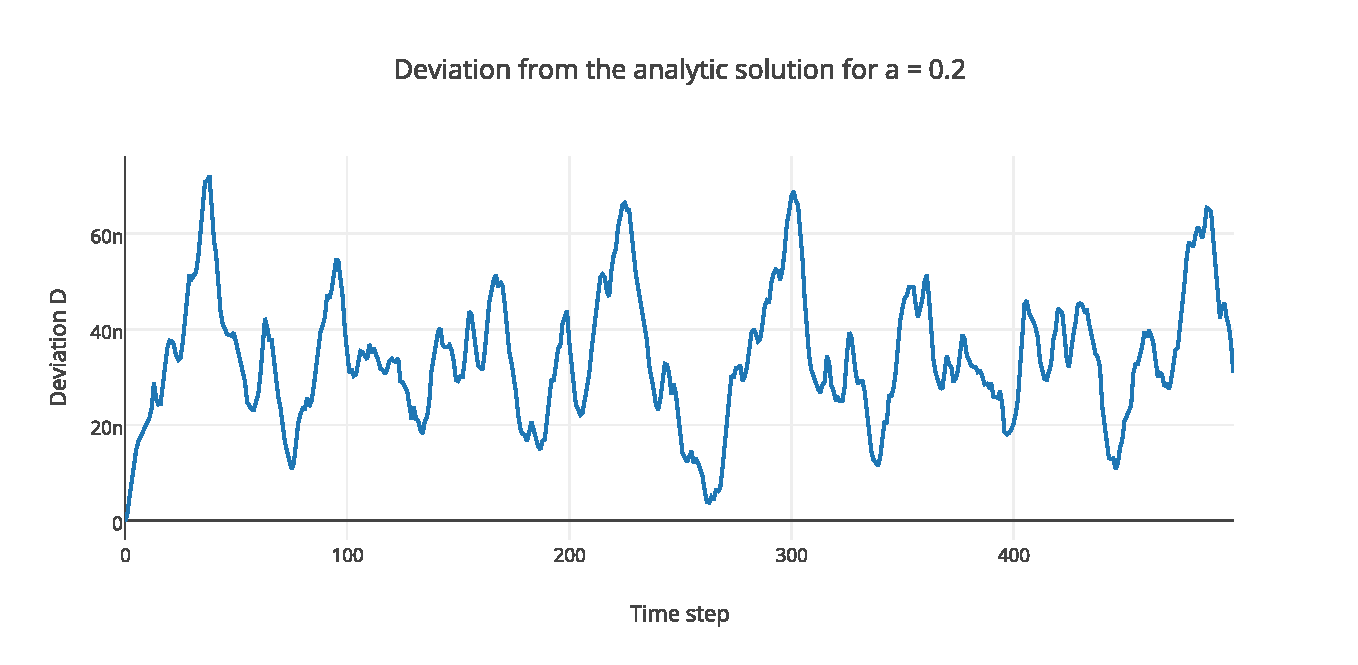
\includegraphics[width=\linewidth]{distancea10.pdf}
    \captionof{figure}{Deviation for each timestep for $a = 1.0$}
    \label{fig:distancea10}
\end{Figure}


\begin{Figure}
    \centering
    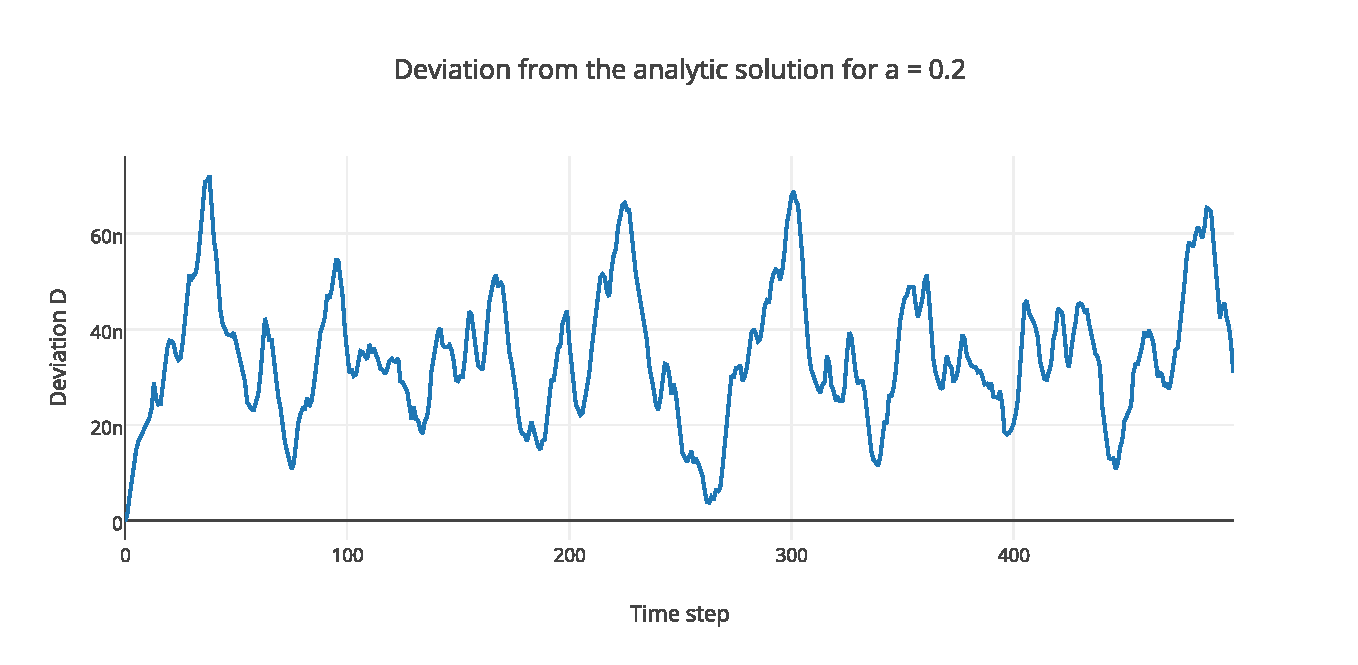
\includegraphics[width=\linewidth]{distancea10.pdf}
    \captionof{figure}{Deviation for each timestep for $a = 0.5$}
    \label{fig:distancea05}
\end{Figure}


\begin{Figure}
    \centering
    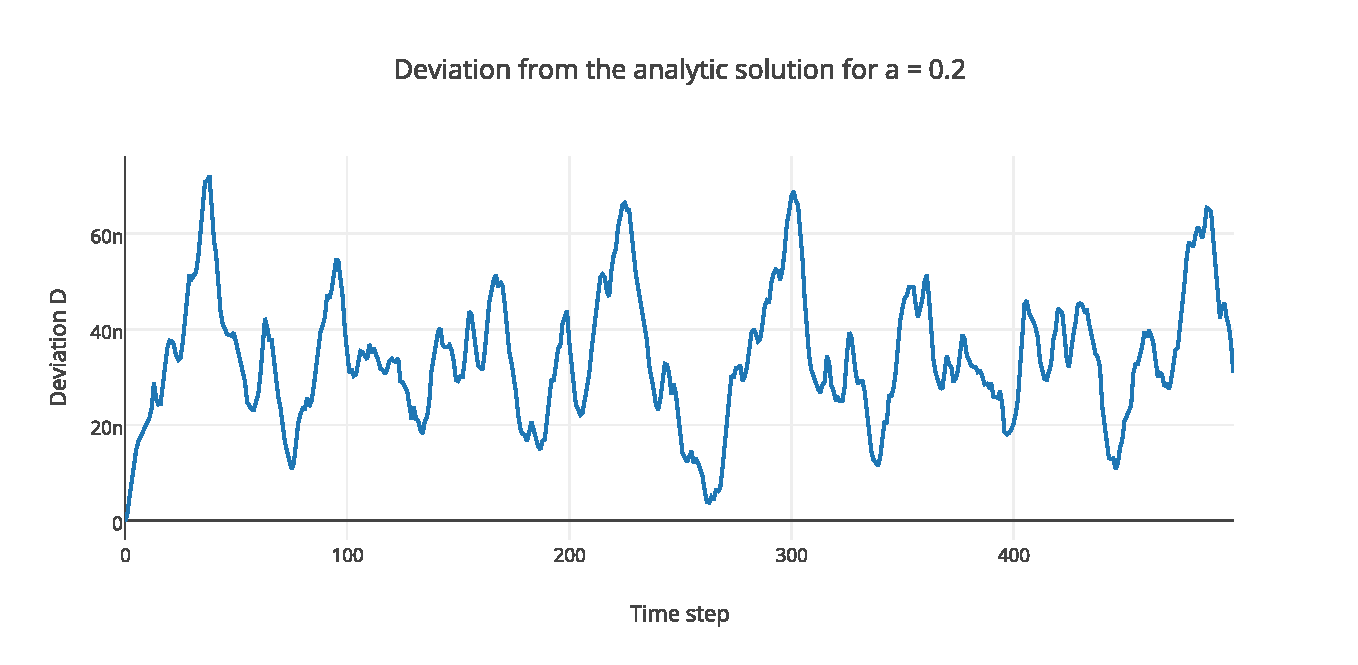
\includegraphics[width=\linewidth]{distancea10.pdf}
    \captionof{figure}{Deviation for each timestep for $a = 0.2$}
    \label{fig:distancea02}
\end{Figure}

The deviations are clearly dependent on the value chosen for $a$, but the running time is expected to be around $\mathcal{O}(a^2)$, so that a proper value of $a$ should be chosen depending on the desired accuracy and running time of the simulation. The deviations occur primarily due to the fact that the analytic eigenstates of the Hamiltonian are not eigenstates of the discretized Hamiltonian\footnote{When the operator $\frac{\mathbb{1}-\frac{i\tau}{2}\hat{H}}{\mathbb{1}+\frac{i\tau}{2}\hat{H}}$ is explicitly calculated, it is possible to find approximate or exact eigenstates of the discretized Hamiltonian.}. The oscillations seen independent of $a$ indicate that the analytic eigenstate and the eigenstate of the discretized Hamiltonian are relatively close with respect to the natural metric.


The norm is seen to change linearly in time. While the change in the norm decreases with decreasing $a$, the total change is neglible except for extremely long simulations, especially since the Schr\"{o}dinger equation and the equations solved in CNM are linear.
